\documentclass[12pt]{article}
\usepackage{amsmath}
\usepackage{graphicx}
\usepackage{float}

\begin{document}

\title{Instacart Model}
\author{Joey Sham}

\maketitle

\section{Introduction}
The following document is a detailed description on the methods used to build the model for the Instacart Kaggle Competition, as well as motivation for features.


\section{How It Works}

\subsection{Given Files}
There were 7 files given:
\begin{itemize}
\item \texttt{aisles}
\item \texttt{departments}
\item \texttt{order\_products\_\_prior}
\item \texttt{order\_products\_\_train}
\item \texttt{orders}
\item \texttt{products}
\item \texttt{sample\_submission}
\end{itemize}

The \texttt{orders} file lists every user, and every order each user has made. There are detailed information such as the day-of-the-week the order was placed, and the sequence of the orders. This allows insight on which products were ordered recently, and which were ordered some time ago.
\newline\newline
The files \texttt{order\_products\_\_prior} and \texttt{order\_products\_\_train} are the exact same format, as they are from the same set of data that has been divided up to \textit{prior} and \textit{train}. The \texttt{order\_products\_\_*} files has detailed information on each order, including what products were ordered in each order, the order in which they were placed into the cart, and a binary value on whether each product has been ordered previously. These files can be joined with the \texttt{orders} file, as \texttt{orders} has column \texttt{eval\_set} with values \textit{prior} or \textit{train} to indicate how the join should happen.
\newline\newline
In this analysis, we will not be using \texttt{aisles} and \texttt{departments}.
\newline\newline
To get all of the files, a new method called \textbf{readFiles} from the file \texttt{pandabase.py} was created to read all the files from the \textbf{/data} folder. This \textbf{/data} folder was not included in the repository due to memory limits.

\subsection{Initial Analysis}
The files are arranged in a very tabular manner, with strong similarity to relational database tables. That means if further analysis is requirement, it may be wise to load the information into a SQL database. Due to time constrant, the files were just loaded in memory into \textbf{DataFrames} via \textbf{pandas} in \textbf{python3}.
\newline\newline
Even after loading the data, it is obviously that the given fields are not enough to create a model. Thus, feature engineering is required which involves creating new columns in the dataframe based on existing data. Features are divided into two sections: user-based features, and product-based features.

\subsection{Feature Engineering} \label{feature_engineering}
Before any new columns are created, a new DataFrame called \texttt{orders\_details\_\_prior} was created by joining/merging \texttt{order\_products\_\_prior} and \texttt{orders} on \texttt{order\_id}. This dataframe is a detailed view of all users and all their orders, with information on which products occured in which order.
\newline
\newline
A new feature called \texttt{no\_of\_times\_user\_bought\_item} is created in \texttt{orders\_details\_\_prior} that counts the total number of times a user has ordered that specific item.

\subsubsection{User-based Features} \label{user_features}
The following is a list of each feature generated based on user behaviour, with a description of the meaning of each feature to each user. A SQL interpretation of this is $GROUP\ BY\ user\_id$.
\newline
\newline
{\textbf{total\_orders}}
\newline
The total number of orders each user has made. Instead of counting, since \texttt{order\_number} exists, this is the equivalent to the \textbf{MAX(\texttt{order\_number})}
\newline
\newline
{\textbf{total\_days\_between\_orders}}
\newline
Sums up the number of days between orders, to get a number representing the total number of days between orders for each user
\newline
\newline
{\textbf{avg\_days\_between\_orders}}
\newline
Takes the mean of number of days between orders, to understand on average how long it takes for each user to make a new order
\newline
\newline
{\textbf{reorder\_ratio\_user}}
\newline
For each user, the \texttt{reorder\_ratio\_user} is calculated with
\begin{equation}
    \begin{split}
    &\frac{number\ of\ reorders\ in\ orders}{number\ of\ products\ ordered\ that's\ not\ in\ the\ first\ order} \\ \\
    &= \frac{count\ all\ orders\ where\ reordered\ == 1}{count\ all\ where\ order\_ number > 1}
    \end{split}
\end{equation}
\newline
\newline
{\textbf{total\_products}}
\newline
Counts the number of products each user has purchased. This is the equivalent to a \textbf{COUNT()} in SQL
\newline
\newline
{\textbf{distinct\_products}}
\newline
Counts the number of distinct/unique products each user has purchased. This is the equivalent to a \textbf{COUNT(DISTINCT())} in SQL
\newline
\newline
{\textbf{average\_no\_items\_per\_order}}
\newline
For each user, the \texttt{average\_no\_items\_per\_order} is calculated by
\begin{equation}
    \frac
    {total\_products}
    {total\_orders}
\end{equation}
which calculates the average number of items in the cart when the user orders
\newline
\newline

\subsubsection{Product-based Features} \label{product_features}
The following is a list of each feature generated based on products, with a description of the meaning of each feature to each product. A SQL interpretation of this is $GROUP\ BY\ product\_id$.
\newline\newline
{\textbf{no\_purchased}}
\newline
The number of times this product has been purchased by users. Note that this count is non-unique, but rather it is the equivalent to a \textbf{COUNT()} in SQL
\newline\newline
{\textbf{no\_reordered}}
\newline
The number of times this order has been reordered. Since \texttt{reordered} is a binary of 0 or 1, this sums the column to get the count.
\newline\newline
{\textbf{no\_bought\_first\_time}}
\newline
The number of times a product is bought the first time by a user. An interpretation of this is the number unique users has bought this item. This counts the number of times \texttt{no\_of\_times\_user\_bought\_item} == 1
\newline\newline
{\textbf{no\_bought\_second\_time}}
\newline
The number of times a product is bought the second time by a user. An interpretation of this is the number of unique users that has bought this item a second time. This counts the number of times \texttt{no\_of\_times\_user\_bought\_item} == 2
\newline\newline
{\textbf{reorder\_prob}}
\newline
This describes the probability that the product will be reordered for a second purchase after a user has bought it the first time. This is calculated by
\begin{equation}
    \begin{split}
        &\frac
        {number\ of\ times\ this\ item\ has\ been\ bought\ a\ second\ time}
        {number\ of\ times\ this\ item\ has\ been\ bought\ the\ first\ time}\\
        = &\frac
        {no\_bought\_first\_time}
        {no\_bought\_second\_time}
    \end{split}
\end{equation}
\newline\newline
{\textbf{reorder\_ratio\_prod}}
\newline
This is the ratio of how many reorders for each item, compared to number of orders. This is calculated by 
This describes the probability that the product will be reordered for a second purchase after a user has bought it the first time. This is calculated by
\begin{equation}
    \begin{split}
        &\frac
        {number\ of\ reorders}
        {number\ of\ purchases}\\
        = &\frac
        {no\_reordered}
        {no\_purchased}
    \end{split}
\end{equation}
\newline\newline
{\textbf{avg\_no\_times\_ordered}}
\newline
This is the average number of times an item is ordered. This is calculated by 
\begin{equation}
    \begin{split}
        &\frac
        {no\_purchased}
        {no\_bought\_first\_time}\\
        =1 + &\frac
        {no\_reordered}
        {no\_bought\_first\_time}
    \end{split}
\end{equation}

\subsubsection{User-based and Product-based Features} \label{user_product_features}
The following is a list of each feature generated based on both users and products, with a description of the meaning of each feature to each user and each product. A SQL interpretation of this is $GROUP\ BY\ user\_id, product\_id$.
\newline\newline
{\textbf{no\_of\_orders}}
\newline
This shows the number of times each user has ordered each product
\newline\newline
{\textbf{order\_number\_of\_first\_purchase}}
\newline
For each user, this displays which order number in their history that they first ordered an item. For example, user with id 1 ordered product 10326 the first time during user 1's 5th order. This can be calcaulted by taking the MIN of \texttt{order\_number}.
\newline\newline
{\textbf{order\_number\_of\_last\_purchase}}
\newline
For each user, this displays which order number in their history that they last ordered an item. For example, user with id 1 ordered product 10326 the last time during user 1's 5th order. As this is the same user from the example above, it can seen that he/she has only ordered this item once. This can be calcaulted by taking the MAX of \texttt{order\_number}.
\newline\newline
{\textbf{avg\_cart\_order\_number}}
\newline
For each user, this describes the average order the product is added to cart.
\newline\newline
{\textbf{order\_rate}}
\newline
This describes how often the user orders this product. This is calculated by
\begin{equation}
    \frac
    {no\_of\_orders}
    {total\_orders}
\end{equation}
\newline\newline
{\textbf{no\_of\_orders\_since\_last\_purchase}}
\newline
This describes how many order it has been since the user has last ordered this specific product. This is calculated by
\begin{equation}
    total\_orders - order\_number\_of\_last\_purchase
\end{equation}
\newline\newline
{\textbf{order\_rate\_since\_first\_purchase}}
\newline
This describes how often this product is ordered since the first purchase of this specific product. This is calculated by
\begin{equation}
    \frac{no\_of\_orders}{total\_orders - order\_number\_of\_first\_purchase + 1}
\end{equation}

\subsection{Model}
Due to the nature of the data, XGBoost was selected to be used to train and generate the model. This falls inline with Instacart's data science team, who also admits to currently using XGBoost. 
\newline\newline
Before training occurs, the data has to be split up. By merging the various dataframes, there exists one dataframe with all relevant information and features that was described in section \ref{feature_engineering}. This dataframe also inherited the \texttt{eval\_set} column from \texttt{orders} file that only has two values: \textit{train} and \textit{test}. From hereon, training data refers to the dataset with $eval\_set = train$ and testing data refers to the dataset with $eval\_set = test$.

\subsubsection{Training}
The idea for training this model is the same as training any other model. Given $x, y$, there exist a process to continuous update $A$ such that $y = Ax$, where $x$ is the input and $y$ is the output. In this scenario, the output is the \texttt{reordered} column, where it has a binary result of $0$ or $1$. The training input data should only contain relevant columns as to eliminate noise and not confuse the learning method. Therefore, columns such as \texttt{eval\_set}, \texttt{user\_id}, \texttt{product\_id}, and \texttt{order\_id} are dropped since their values do not directly contribute to the binary result of \texttt{reordered}.
\newline\newline
At this point, there are two dataframes: \texttt{X\_train} for training data $x$, and \texttt{y\_train} for training \texttt{reordered} data $y$. These two dataframes are fed into the XGBoost training object, with different hyperparameters. Selection of hyperparameters is sometimes more of an art than a science, and can be time consuming since each epoch takes quite a bit of time. The most important part is to know the objective is "reg:logistic" as this is a classification problem. It is common to use logloss as an evaluation metric, as rmse and mae can incurr L1 and L2 errors.

\begin{figure}[H]
    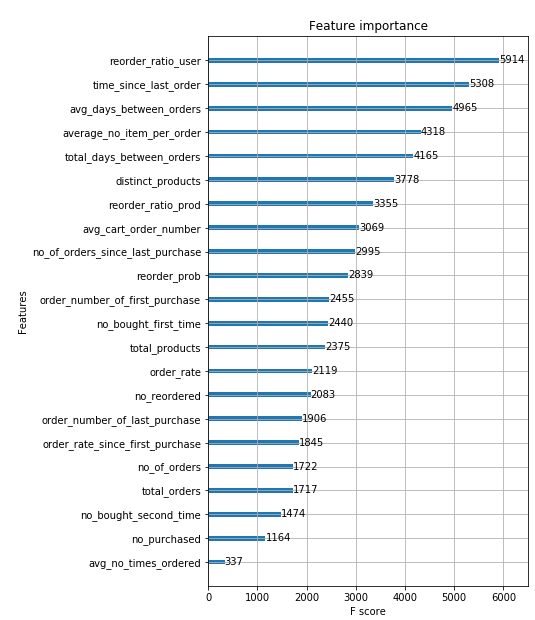
\includegraphics[width=\linewidth]{feature_importance.png}
    \caption{XGBoost Training Feature Importance}
    \label{fig:feat_imp}
\end{figure}

After training, it is often beneficial to view which features contribute to the training model the most, especially when there is an increasing number of features. Figure (\ref{fig:feat_imp}) above shows a graph comparing the features described above, ordered from highest attribution to the model to the least.

\subsubsection{Predicting}
Similar to creating a dataframe for training, the test input data has to drop irrelevant columns. This include columns such as \texttt{eval\_set}, \texttt{user\_id}, \texttt{product\_id}, \texttt{reordered}, and \texttt{order\_id}. \texttt{reordered} is dropped in the testing dataframe because this is the desired output, and should not be a part of the input. The resulting dataframe can be input into the XGBoost trained model.
\newline\newline
From the testing data, all predicted score above 0.21 are considered to be reordered, and below is not. The results are aggregated and appended to the \texttt{sample\_submission} file. The dataframe is aggregated in such a way that for every \texttt{order\_id}, \texttt{products} column has the \texttt{product\_id} where \texttt{reordered} was calculated to be 1. For example, the dataframe would be of the form

\begin{center}
\begin{tabular}{ c l }
 order\_id & products \\ 
 \hline
 17 & 13107 21463 \\  
 34 & 47792
\end{tabular}
\end{center}

\section{Result}
While there is some variability in the submissions, the submission score is \textbf{0.3812513}.

\section{Future Improvements}
There are two major ways to improve the model. The first is to create new features, and the second is to tune the hyperparameters. There are a lot of literature out there that describes how better to tune hyperparameters, so it will not be discussed here. Creation of new features would be an interesting task, and the feature importance plot can be used to determine how well various engineered features fare. One of these possible features could be one that integrates recency, such that if products were heavily ordered in orders 1-5, but not ordered in orders 6-9, then it can help determine such a product would be less likely to be reordered. 


\begin{figure}[H]
    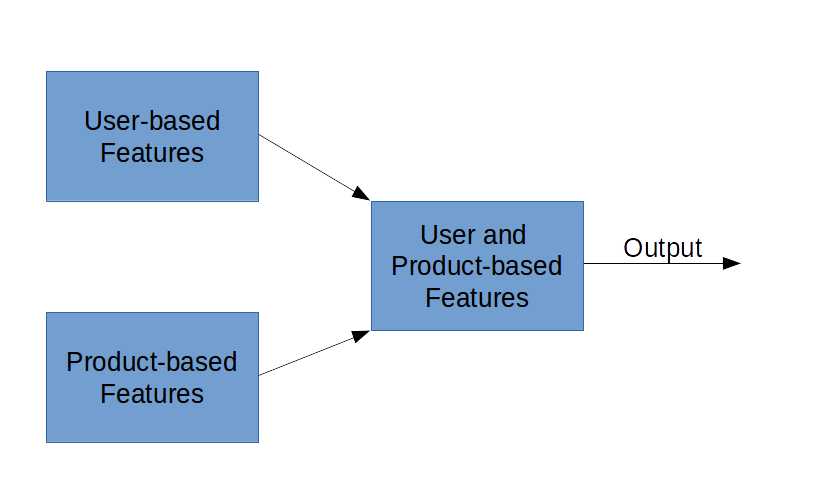
\includegraphics[width=\linewidth]{future_model.png}
    \caption{Future Model Design}
    \label{fig:future_model}
\end{figure}

As described above, the features are divided into user-based (see Section \ref{user_features}) and product-based (see Section \ref{product_features}). A possible next step could be to divide up the features into two separate dataframes, each fed into its own model, and combine the results. Then there would be a user-specific model, and a product-specific model, and both would merge into a user-product-model with user-product features (see Section \ref{user_product_features}). An example of that can be seen in the figure \ref{fig:future_model} above.

\end{document}
